\documentclass[a3paper]{article}
\usepackage[utf8]{inputenc}
\usepackage[margin=0.8in]{geometry}

\usepackage{tikz}
\usetikzlibrary{arrows,positioning,shapes.geometric,calc, shapes, shapes.gates.logic.US}

\title{Attack Tools}

\tikzset{
 	headerblock/.style= {draw=none, rectangle, align=center,minimum width=2.5cm,minimum height=0.75cm, fill=gray!30, font=\bf}, 
 	block/.style= {draw, rectangle, align=center,minimum width=2.4cm,minimum height=0.5cm, font=\bfseries}
 }
 
\def \largeX {18cm}
\def \smallY {0.1cm}

\begin{document}
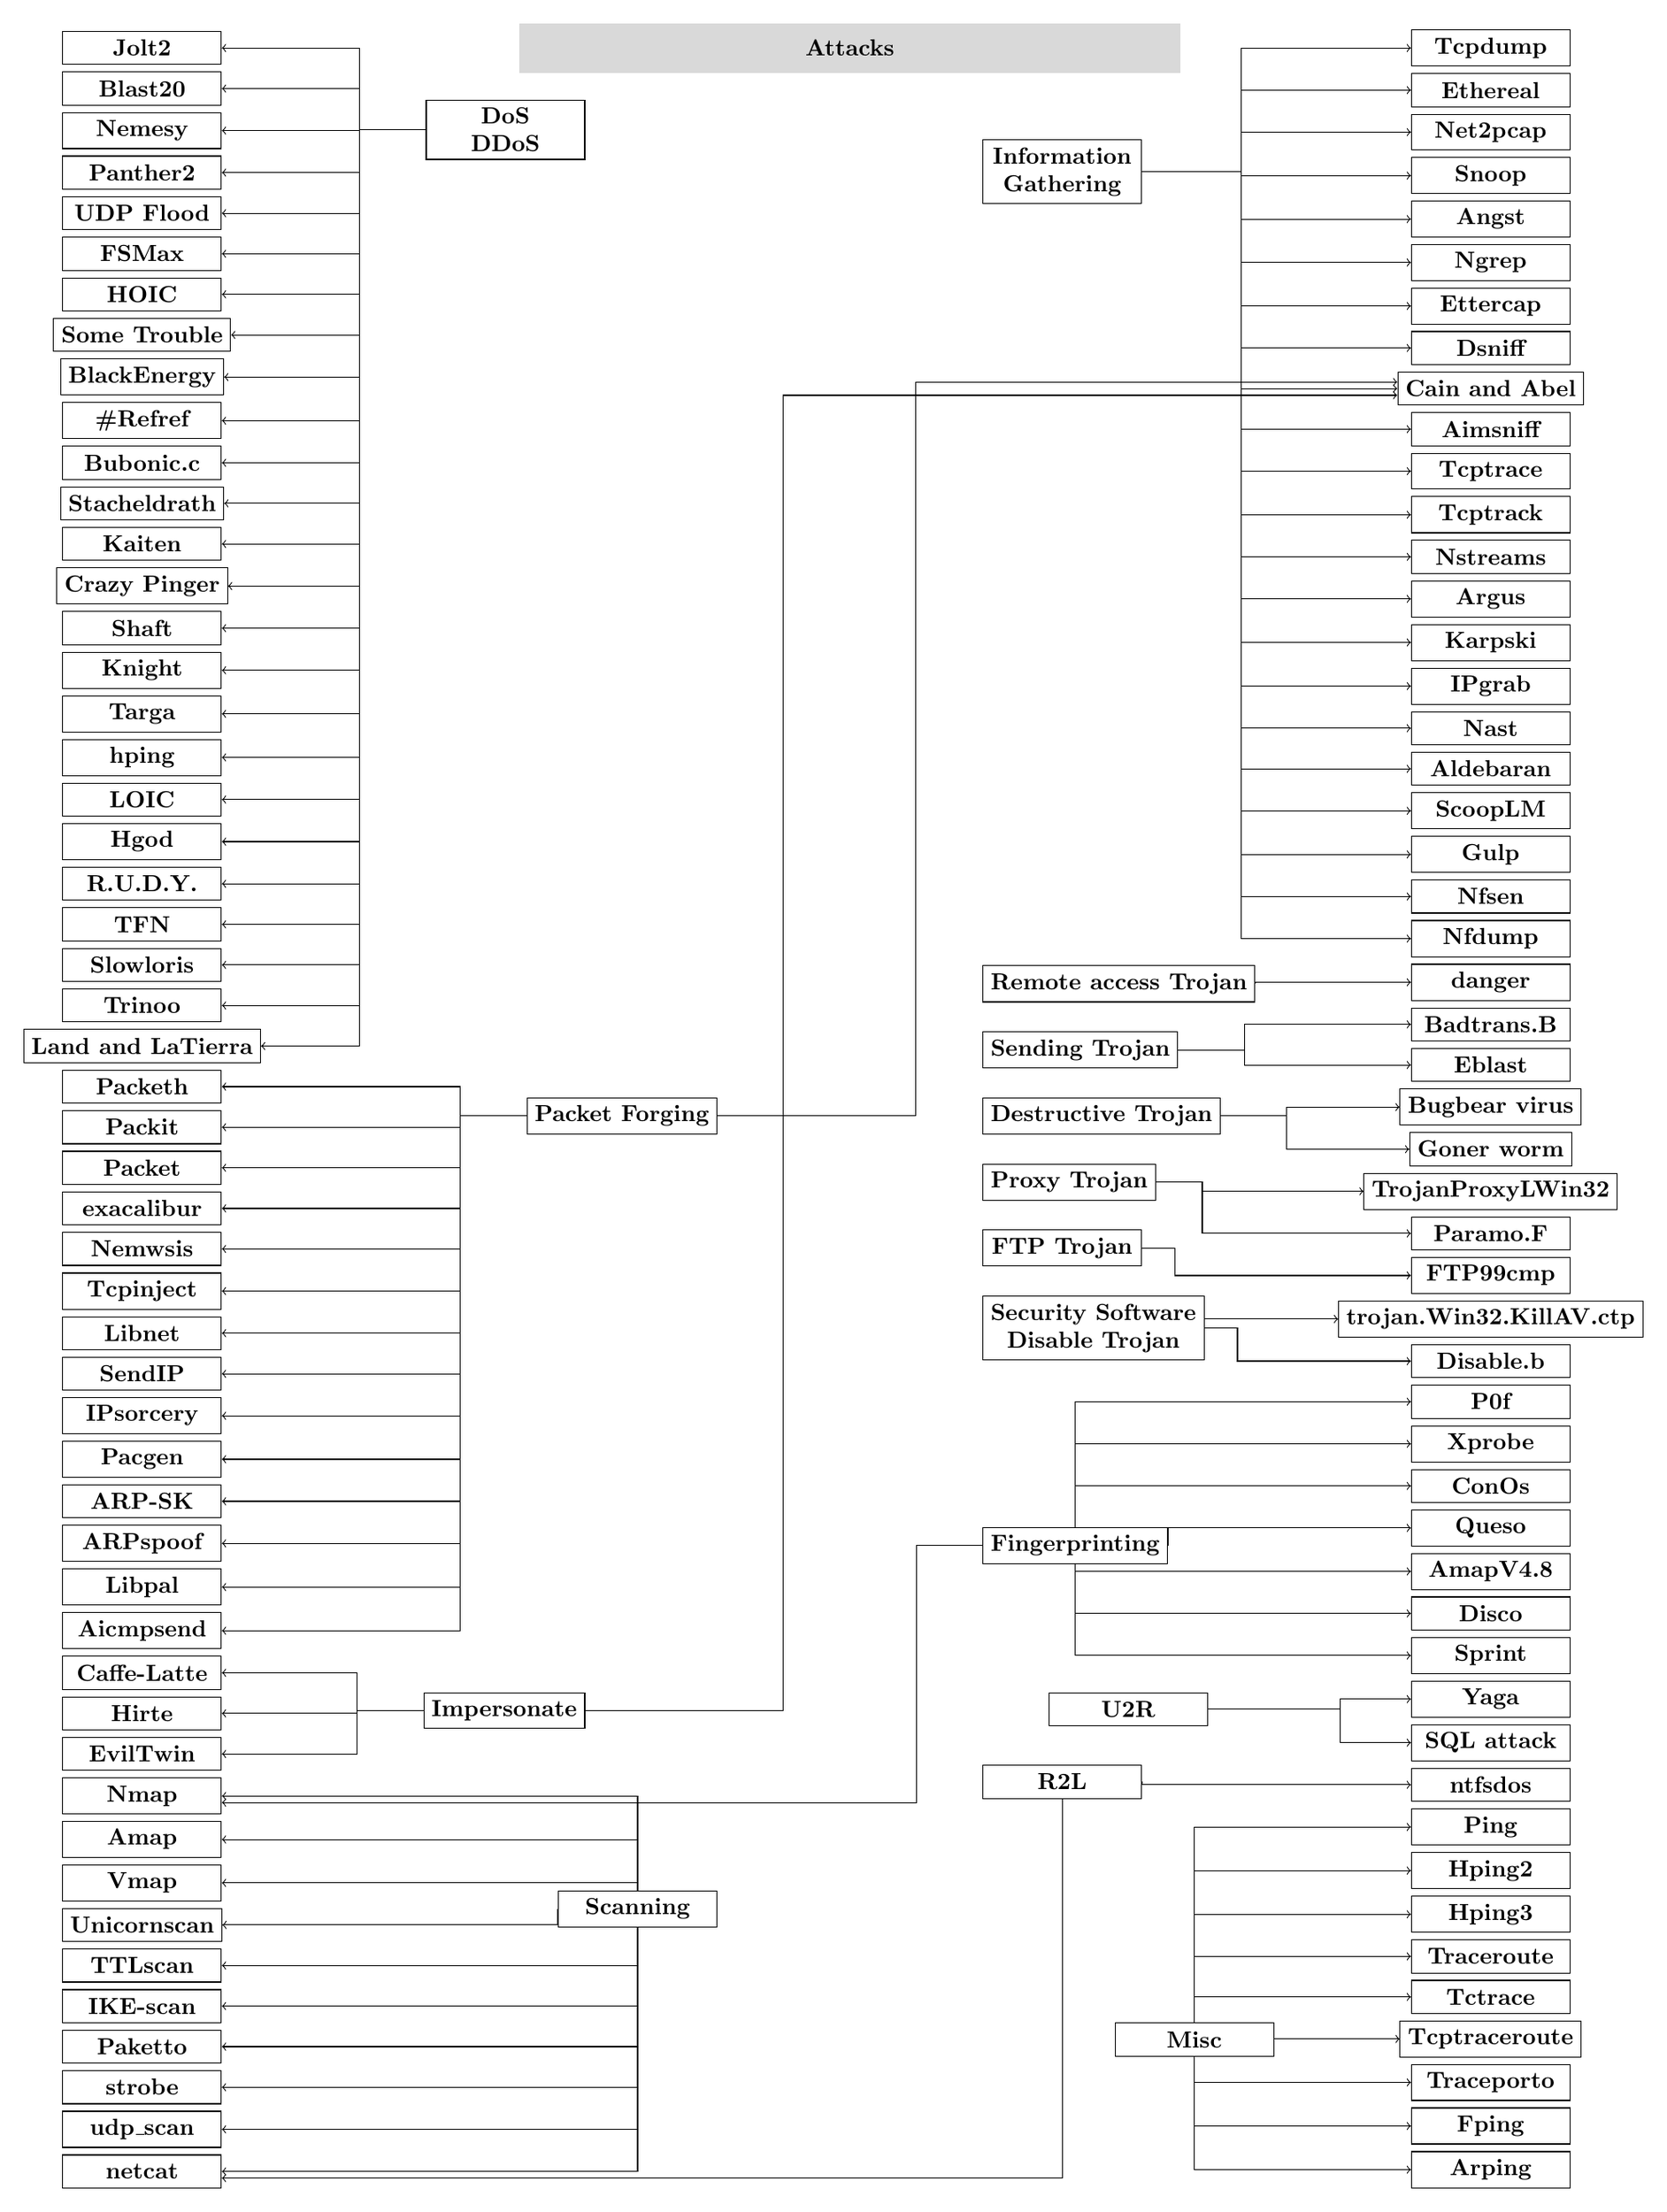
\begin{tikzpicture}
%%%%%%%%%%%%%%%%%%%%% Left Column %%%%%%%%%%%%%%%%%%%%%
    \node [block] (a1) {Jolt2};
    \node [block, below = \smallY of a1] (a2) {Blast20};
    \node [block, below = \smallY of a2] (a3) {Nemesy};
    \node [block, below = \smallY of a3] (a4) {Panther2};
    \node [block, below = \smallY of a4] (a5) {UDP Flood};
    \node [block, below = \smallY of a5] (a6) {FSMax};
    \node [block, below = \smallY of a6] (a7) {HOIC};
    \node [block, below = \smallY of a7] (a8) {Some Trouble};
    \node [block, below = \smallY of a8] (a9) {BlackEnergy};
    \node [block, below = \smallY of a9] (a10) {\#Refref};
    \node [block, below = \smallY of a10] (a11) {Bubonic.c};
    \node [block, below = \smallY of a11] (a12) {Stacheldrath};
    \node [block, below = \smallY of a12] (a13) {Kaiten};
    \node [block, below = \smallY of a13] (a14) {Crazy Pinger};
    \node [block, below = \smallY of a14] (a15) {Shaft};
    \node [block, below = \smallY of a15] (a16) {Knight};
    \node [block, below = \smallY of a16] (a17) {Targa};
    \node [block, below = \smallY of a17] (a18) {hping};
    \node [block, below = \smallY of a18] (a19) {LOIC};
    \node [block, below = \smallY of a19] (a20) {Hgod};
    \node [block, below = \smallY of a20] (a21) {R.U.D.Y.};
    \node [block, below = \smallY of a21] (a22) {TFN};
    \node [block, below = \smallY of a22] (a23) {Slowloris};
    \node [block, below = \smallY of a23] (a24) {Trinoo};
    \node [block, below = \smallY of a24] (a25) {Land and LaTierra};
    \node [block, below = \smallY of a25] (a26) {Packeth};
    \node [block, below = \smallY of a26] (a27) {Packit};
    \node [block, below = \smallY of a27] (a28) {Packet};
    \node [block, below = \smallY of a28] (a29) {exacalibur};
    \node [block, below = \smallY of a29] (a30) {Nemwsis};
    \node [block, below = \smallY of a30] (a31) {Tcpinject};
    \node [block, below = \smallY of a31] (a32) {Libnet};
    \node [block, below = \smallY of a32] (a33) {SendIP};
    \node [block, below = \smallY of a33] (a34) {IPsorcery};
    \node [block, below = \smallY of a34] (a35) {Pacgen};
    \node [block, below = \smallY of a35] (a36) {ARP-SK};
    \node [block, below = \smallY of a36] (a37) {ARPspoof};
    \node [block, below = \smallY of a37] (a38) {Libpal};
    \node [block, below = \smallY of a38] (a39) {Aicmpsend};
    \node [block, below = \smallY of a39] (a40) {Caffe-Latte};
    \node [block, below = \smallY of a40] (a41) {Hirte};
    \node [block, below = \smallY of a41] (a42) {EvilTwin};
    \node [block, below = \smallY of a42] (a43) {Nmap};
    \node [block, below = \smallY of a43] (a44) {Amap};
    \node [block, below = \smallY of a44] (a45) {Vmap};
    \node [block, below = \smallY of a45] (a46) {Unicornscan};
    \node [block, below = \smallY of a46] (a47) {TTLscan};
    \node [block, below = \smallY of a47] (a48) {IKE-scan};
    \node [block, below = \smallY of a48] (a49) {Paketto};
    \node [block, below = \smallY of a49] (a50) {strobe};
    \node [block, below = \smallY of a50] (a51) {udp\_scan};
    \node [block, below = \smallY of a51] (a52) {netcat};

%%%%%%%%%%%%%%%%%%%%% Right Column %%%%%%%%%%%%%%%%%%%%%
    \node [block, right=\largeX of a1] (b1) {Tcpdump};
    \node [block, below = \smallY of b1] (b2) {Ethereal};
    \node [block, below = \smallY of b2] (b3) {Net2pcap};
    \node [block, below = \smallY of b3] (b4) {Snoop};
    \node [block, below = \smallY of b4] (b5) {Angst};
    \node [block, below = \smallY of b5] (b6) {Ngrep};
    \node [block, below = \smallY of b6] (b7) {Ettercap};
    \node [block, below = \smallY of b7] (b8) {Dsniff};
    \node [block, below = \smallY of b8] (b9) {Cain and Abel};
    \node [block, below = \smallY of b9] (b10) {Aimsniff};
    \node [block, below = \smallY of b10] (b11) {Tcptrace};
    \node [block, below = \smallY of b11] (b12) {Tcptrack};
    \node [block, below = \smallY of b12] (b13) {Nstreams};
    \node [block, below = \smallY of b13] (b14) {Argus};
    \node [block, below = \smallY of b14] (b15) {Karpski};
    \node [block, below = \smallY of b15] (b16) {IPgrab};
    \node [block, below = \smallY of b16] (b17) {Nast};
    \node [block, below = \smallY of b17] (b18) {Aldebaran};
    \node [block, below = \smallY of b18] (b19) {ScoopLM};
    \node [block, below = \smallY of b19] (b20) {Gulp};
    \node [block, below = \smallY of b20] (b21) {Nfsen};
    \node [block, below = \smallY of b21] (b22) {Nfdump};
    \node [block, below = \smallY of b22] (b23) {danger};
    \node [block, below = \smallY of b23] (b24) {Badtrans.B};
    \node [block, below = \smallY of b24] (b25) {Eblast};
    \node [block, below = \smallY of b25] (b26) {Bugbear virus};
    \node [block, below = \smallY of b26] (b27) {Goner worm};
    \node [block, below = \smallY of b27] (b28) {TrojanProxyLWin32};
    \node [block, below = \smallY of b28] (b29) {Paramo.F};
    \node [block, below = \smallY of b29] (b30) {FTP99cmp};
    \node [block, below = \smallY of b30] (b31) {trojan.Win32.KillAV.ctp};
    \node [block, below = \smallY of b31] (b32) {Disable.b};
    \node [block, below = \smallY of b32] (b33) {P0f};
    \node [block, below = \smallY of b33] (b34) {Xprobe};
    \node [block, below = \smallY of b34] (b35) {ConOs};
    \node [block, below = \smallY of b35] (b36) {Queso};
    \node [block, below = \smallY of b36] (b37) {AmapV4.8};
    \node [block, below = \smallY of b37] (b38) {Disco};
    \node [block, below = \smallY of b38] (b39) {Sprint};
    \node [block, below = \smallY of b39] (b40) {Yaga};
    \node [block, below = \smallY of b40] (b41) {SQL attack};
    \node [block, below = \smallY of b41] (b42) {ntfsdos};
    \node [block, below = \smallY of b42] (b43) {Ping};
    \node [block, below = \smallY of b43] (b44) {Hping2};
    \node [block, below = \smallY of b44] (b45) {Hping3};
    \node [block, below = \smallY of b45] (b46) {Traceroute};
    \node [block, below = \smallY of b46] (b47) {Tctrace};
    \node [block, below = \smallY of b47] (b48) {Tcptraceroute};
    \node [block, below = \smallY of b48] (b49) {Traceporto};
    \node [block, below = \smallY of b49] (b50) {Fping};
    \node [block, below = \smallY of b50] (b51) {Arping};

%%%%%%%%%%%%%%%%%%%%% Attacks %%%%%%%%%%%%%%%%%%%%%
    \node [headerblock, right = \largeX/4 of a1, minimum width = 10cm] (attacks) {\textbf{Attacks}};
    \node [block, below left = \smallY*4 and \smallY*-10 of attacks] (dos) {DoS\\DDoS};  
    \node [block, below right = \smallY*10 and \smallY*-30 of attacks] (info) {Information\\Gathering};
    \node [block, below right = \smallY*135 and \smallY*-30 of attacks] (remote) {Remote access Trojan};
    \node [block, below right = \smallY*145 and \smallY*-30 of attacks] (sending) {Sending Trojan};
    \node [block, below right = \smallY*155 and \smallY*-30 of attacks] (destructive) {Destructive Trojan};
    \node [block, block, below right = \smallY*165 and \smallY*-30 of attacks] (proxy) {Proxy Trojan};
    \node [block, block, below right = \smallY*175 and \smallY*-30 of attacks] (ftp) {FTP Trojan};
    \node [block, block, below right = \smallY*185 and \smallY*-30 of attacks] (disable) {Security Software\\Disable Trojan};
    \node [block, block, below left = \smallY*155 and \smallY*-30 of attacks] (forging) {Packet Forging};
    \node [block, block, below right = \smallY*220 and \smallY*-30 of attacks] (fingerprinting) {Fingerprinting};
    \node [block, block, below right = \smallY*245 and \smallY*-20 of attacks] (u2r) {U2R};
    \node [block, block, below left = \smallY*245 and \smallY*-10 of attacks] (impersonate) {Impersonate};
    \node [block, block, below right = \smallY*256 and \smallY*-30 of attacks] (r2l) {R2L};
    \node [block, block, below left = \smallY*275 and \smallY*-30 of attacks] (scanning) {Scanning};
    \node [block, block, below right = \smallY*295 and \smallY*-10 of attacks] (misc) {Misc};

%%%%%%%%%%%%%%%%%%%%%%%%%%%%%%%%%%%%%%%%%%%%%%%%%
%%%%%%%%%%%%%%%%%%%%% Links %%%%%%%%%%%%%%%%%%%%%
%%%%%%%%%%%%%%%%%%%%%%%%%%%%%%%%%%%%%%%%%%%%%%%%%

	%DoS
	\draw[->] (dos.west) -- ($(dos.west) - (1, 0)$)  |- (a1.east); 
    \draw[->] (dos.west) -- ($(dos.west) - (1, 0)$)  |- (a2.east); 
    \draw[->] (dos.west) -- ($(dos.west) - (1, 0)$)  |- (a3.east); 
   	\draw[->] (dos.west) -- ($(dos.west) - (1, 0)$)  |- (a4.east);
   	\draw[->] (dos.west) -- ($(dos.west) - (1, 0)$)  |- (a5.east);
   	\draw[->] (dos.west) -- ($(dos.west) - (1, 0)$)  |- (a6.east);
   	\draw[->] (dos.west) -- ($(dos.west) - (1, 0)$)  |- (a7.east);
   	\draw[->] (dos.west) -- ($(dos.west) - (1, 0)$)  |- (a8.east);
   	\draw[->] (dos.west) -- ($(dos.west) - (1, 0)$)  |- (a9.east);
   	\draw[->] (dos.west) -- ($(dos.west) - (1, 0)$)  |- (a10.east);
   	\draw[->] (dos.west) -- ($(dos.west) - (1, 0)$)  |- (a11.east);
   	\draw[->] (dos.west) -- ($(dos.west) - (1, 0)$)  |- (a12.east);
   	\draw[->] (dos.west) -- ($(dos.west) - (1, 0)$)  |- (a13.east);
   	\draw[->] (dos.west) -- ($(dos.west) - (1, 0)$)  |- (a14.east);
   	\draw[->] (dos.west) -- ($(dos.west) - (1, 0)$)  |- (a15.east);
   	\draw[->] (dos.west) -- ($(dos.west) - (1, 0)$)  |- (a16.east);
   	\draw[->] (dos.west) -- ($(dos.west) - (1, 0)$)  |- (a17.east);
   	\draw[->] (dos.west) -- ($(dos.west) - (1, 0)$)  |- (a18.east);
   	\draw[->] (dos.west) -- ($(dos.west) - (1, 0)$)  |- (a19.east);
   	\draw[->] (dos.west) -- ($(dos.west) - (1, 0)$)  |- (a20.east);
   	\draw[->] (dos.west) -- ($(dos.west) - (1, 0)$)  |- (a21.east);
   	\draw[->] (dos.west) -- ($(dos.west) - (1, 0)$)  |- (a22.east);
   	\draw[->] (dos.west) -- ($(dos.west) - (1, 0)$)  |- (a23.east);
   	\draw[->] (dos.west) -- ($(dos.west) - (1, 0)$)  |- (a24.east);
   	\draw[->] (dos.west) -- ($(dos.west) - (1, 0)$)  |- (a25.east);
   
   	% forging 
    \draw[->] (forging.west) -- ($(forging.west) - (1, 0)$)  |- (a26.east);
    \draw[->] (forging.west) -- ($(forging.west) - (1, 0)$)  |- (a27.east);
    \draw[->] (forging.west) -- ($(forging.west) - (1, 0)$)  |- (a28.east);
    \draw[->] (forging.west) -- ($(forging.west) - (1, 0)$)  |- (a29.east);
    \draw[->] (forging.west) -- ($(forging.west) - (1, 0)$)  |- (a30.east);
    \draw[->] (forging.west) -- ($(forging.west) - (1, 0)$)  |- (a31.east);
    \draw[->] (forging.west) -- ($(forging.west) - (1, 0)$)  |- (a32.east);
    \draw[->] (forging.west) -- ($(forging.west) - (1, 0)$)  |- (a33.east);
    \draw[->] (forging.west) -- ($(forging.west) - (1, 0)$)  |- (a34.east);
    \draw[->] (forging.west) -- ($(forging.west) - (1, 0)$)  |- (a35.east);
    \draw[->] (forging.west) -- ($(forging.west) - (1, 0)$)  |- (a36.east);
    \draw[->] (forging.west) -- ($(forging.west) - (1, 0)$)  |- (a37.east);
    \draw[->] (forging.west) -- ($(forging.west) - (1, 0)$)  |- (a38.east);
    \draw[->] (forging.west) -- ($(forging.west) - (1, 0)$)  |- (a39.east);
    \draw[->] (forging.east) -- ($(forging.east) - (-3, 0)$) |- ($(b9.west)-(0,-0.1)$); 


	%Information Gathering
    \draw[->] (info.east) -- ($(info.east) - (-1.5, 0)$)  |- (b1.west); 
    \draw[->] (info.east) -- ($(info.east) - (-1.5, 0)$)  |- (b2.west); 
    \draw[->] (info.east) -- ($(info.east) - (-1.5, 0)$)  |- (b3.west);  
    \draw[->] (info.east) -- ($(info.east) - (-1.5, 0)$)  |- (b4.west);  
    \draw[->] (info.east) -- ($(info.east) - (-1.5, 0)$)  |- (b5.west); 
    \draw[->] (info.east) -- ($(info.east) - (-1.5, 0)$)  |- (b6.west); 
    \draw[->] (info.east) -- ($(info.east) - (-1.5, 0)$)  |- (b7.west); 
    \draw[->] (info.east) -- ($(info.east) - (-1.5, 0)$)  |- (b8.west); 
    \draw[->] (info.east) -- ($(info.east) - (-1.5, 0)$)  |- (b9.west); 
    \draw[->] (info.east) -- ($(info.east) - (-1.5, 0)$)  |- (b10.west); 
    \draw[->] (info.east) -- ($(info.east) - (-1.5, 0)$)  |- (b11.west); 
    \draw[->] (info.east) -- ($(info.east) - (-1.5, 0)$)  |- (b12.west); 
    \draw[->] (info.east) -- ($(info.east) - (-1.5, 0)$)  |- (b13.west); 
    \draw[->] (info.east) -- ($(info.east) - (-1.5, 0)$)  |- (b14.west); 
    \draw[->] (info.east) -- ($(info.east) - (-1.5, 0)$)  |- (b15.west); 
    \draw[->] (info.east) -- ($(info.east) - (-1.5, 0)$)  |- (b16.west); 
    \draw[->] (info.east) -- ($(info.east) - (-1.5, 0)$)  |- (b17.west); 
    \draw[->] (info.east) -- ($(info.east) - (-1.5, 0)$)  |- (b18.west); 
    \draw[->] (info.east) -- ($(info.east) - (-1.5, 0)$)  |- (b19.west); 
    \draw[->] (info.east) -- ($(info.east) - (-1.5, 0)$)  |- (b20.west); 
    \draw[->] (info.east) -- ($(info.east) - (-1.5, 0)$)  |- (b21.west); 
    \draw[->] (info.east) -- ($(info.east) - (-1.5, 0)$)  |- (b22.west); 
   
    %Remote Access
    \draw[->] (remote.east) |- (b23.west); 
        
	%Sending
    \draw[->] (sending.east) -- ($(sending.east) - (-1, 0)$) |- (b24.west);
    \draw[->] (sending.east) -- ($(sending.east) - (-1, 0)$) |- (b25.west);
    
	%Destructive
    \draw[->] (destructive.east) -- ($(destructive.east) - (-1, 0)$) |- (b26.west);
    \draw[->] (destructive.east) -- ($(destructive.east) - (-1, 0)$) |- (b27.west);
    
	%Proxy
    \draw[->] (proxy.east) -- ($(proxy.east) - (-0.7, 0)$) |- (b28.west);
    \draw[->] (proxy.east) -- ($(proxy.east) - (-0.7, 0)$) |- (b29.west);
    
    %FTP
    \draw[->] (ftp.east) -- ($(ftp.east) - (-0.5, 0)$) |- (b30.west); 
    
	% disable
    \draw[->] (disable.east) |- (b31.west); 
    \draw[->] (disable.east) -- ($(disable.east) - (-0.5, 0)$) |- (b32.west); 
    
	%Impersonate 
    \draw[->] (impersonate.west) -- ($(impersonate.west) - (1, 0)$) |- (a40.east); 
    \draw[->] (impersonate.west) -- ($(impersonate.west) - (1, 0)$) |- (a41.east); 
    \draw[->] (impersonate.west) -- ($(impersonate.west) - (1, 0)$) |- (a42.east); 
    \draw[->] (impersonate.east) -- ($(impersonate.east) - (-3, 0)$) |- ($(b9.west)-(0,0.1)$); 
    
	%Fingerprinting 
    \draw[->] (fingerprinting.north) |- (b33.west); 
	\draw[->] (fingerprinting.north) |- (b34.west); 
	\draw[->] (fingerprinting.north) |- (b35.west); 
	\draw[->] (fingerprinting.east) |- (b36.west); 
	\draw[->] (fingerprinting.south) |- (b37.west); 
	\draw[->] (fingerprinting.south) |- (b38.west); 
	\draw[->] (fingerprinting.south) |- (b39.west); 
    \draw[->] (fingerprinting.west) -- ($(fingerprinting.west) - (1, 0)$) |- ($(a43.east) - (0,0.1)$); 
    
    
	%Scanning 
    \draw[->] (scanning.north) |- (a43.east); 
    \draw[->] (scanning.north) |- (a44.east); 
    \draw[->] (scanning.north) |- (a45.east); 
    \draw[->] (scanning.west) |- (a46.east); 
    \draw[->] (scanning.south) |- (a47.east); 
	\draw[->] (scanning.south) |- (a48.east); 
    \draw[->] (scanning.south) |- (a49.east); 
    \draw[->] (scanning.south) |- (a50.east); 
    \draw[->] (scanning.south) |- (a51.east); 
	\draw[->] (scanning.south) |- (a52.east); 
    
	%u2L
    \draw[->] (u2r.east) -- ($(u2r.east) - (-2, 0)$) |- (b40.west) ; 
    \draw[->] (u2r.east) -- ($(u2r.east) - (-2, 0)$) |- (b41.west) ; 
    
    %R2L
    \draw[->] (r2l.east) |- (b42.west); 
    \draw[->] (r2l.south) |- ($(a52.east)- (0,0.1)$); 
    
    %Misc
    \draw[->] (misc.north) |- (b43.west); 
    \draw[->] (misc.north) |- (b44.west); 
    \draw[->] (misc.north) |- (b45.west); 
    \draw[->] (misc.north) |- (b46.west); 
    \draw[->] (misc.north) |- (b47.west); 
    \draw[->] (misc.east) |- (b48.west); 
    \draw[->] (misc.south) |- (b49.west); 
    \draw[->] (misc.south) |- (b50.west); 
    \draw[->] (misc.south) |- (b51.west); 

\end{tikzpicture}
\end{document}

